\documentclass[11pt,a4paper]{article}
\usepackage[T1]{fontenc}
\usepackage[utf8]{inputenc}
\usepackage{lmodern}
\usepackage[a4paper,hmargin=23mm,vmargin=21mm]{geometry}
\usepackage{amsmath,amssymb,amsthm,booktabs,tabularx,array}
\usepackage{tikz}
\usetikzlibrary{arrows.meta,positioning,fit,backgrounds,calc}
\usepackage{xurl}
\usepackage[colorlinks,allcolors=blue!55!black]{hyperref}
\renewcommand{\abstractname}{Resumen}
\renewcommand{\figurename}{Figura}
\renewcommand{\tablename}{Tabla}
\renewcommand{\refname}{Referencias}
\renewcommand{\proofname}{Demostración}
\newtheorem{proposition}{Proposición}
\newcommand{\bits}{\{0,1\}}
\newcommand{\hm}{H_{\min}}
\newcommand{\ud}{\mathsf U}
\newcommand{\dist}{\Delta}
\newcommand{\AES}{\operatorname{AES256}}
\newcommand{\SHA}{\operatorname{SHA256}}
\newcommand{\pg}{p_{\mathrm{guess}}}
\newcolumntype{Y}{>{\raggedright\arraybackslash}X}
\title{Un PTRNG PTG.3 con salida ITS\\
\large Toeplitz dentro del PTG.2 y postprocesado biyectivo según AIS 20/31 v3.0}
\author{Nota técnica para Jordi Prieto Gallego}
\date{20 de noviembre de 2026}
\begin{document}
\maketitle
\begin{abstract}
Se especifica una arquitectura candidata a PTG.3 con un PTRNG interno PTG.2,
compresión Toeplitz y el postprocesado con memoria de los §§996--998 de la
referencia AIS 20/31 de 2024. Cada bloque completo de salida consume exactamente
128 bits frescos del PTG.2. Para cada estado, el mapa que genera ese bloque es
una permutación y conserva la minentropía condicional y la distancia a uniforme.
Se construye una Toeplitz fija con una cota explícita bajo un modelo condicional
de bits independientes y se da un método para modelos con dependencia.
Se identifican las obligaciones algorítmicas DRG.3 que cubre el ejemplo de BSI
y la evidencia adicional exigible para evaluar la instancia y el producto.
\end{abstract}

\section{Objetivo y modelo de seguridad}

El PTRNG interno PTG.2 incluye la fuente física, las pruebas sobre muestras
raw y Toeplitz. Entrega 128 bits frescos por llamada al postprocesado con
memoria, que usa AES-256 para la salida y SHA-256 para actualizar el estado.
El objetivo del expediente es PTG.3 con la quinta selección de PTG.3.5
(minentropía concreta por bit de \emph{salida interna}) y un claim técnico ITS
adicional que explicita la información lateral. Como objetivo de diseño se toma
$v_m=1-2^{-32}$, extremo permitido en PTG.3.5. Esta cifra sólo se declara si
el modelo y sus parámetros justifican la cota. La selección básica de
PTG.3.5, con $0.98$ de minentropía por bit intermedio y sin expansión, también
puede formularse si esa es la cota acreditada. El perfil PTG.2 de entrada sigue
siendo PTG.2; el valor adicional que se transfiere a PTG.3 debe respaldarse con
el dossier del modelo y su evidencia. El §398 permite las selecciones
concretas para una biyección, pero su paréntesis da los límites $0.98$ y
$0.9998$, distintos del máximo $1-2^{-32}$ que constan en el SFR del §375
y en la nota del §403. La propuesta toma el intervalo del SFR como base.
El expediente debe señalar la discrepancia y acordar su lectura con el
organismo antes de cerrar el claim concreto
\cite[§§315--319, 375, 395--398 y 403]{ais}.

Denótese $R_i\in\bits^n$ la adquisición raw del bloque $i$,
$A_i=T R_i\in\bits^{128}$ la salida intermedia del PTG.2 y $Y_i$ la salida
interna del PTG.3. $S_i\in\bits^{256}$ es el estado antes de la operación.
$E$ representa una vista declarada del adversario que puede incluir ambiente,
ruido clásico observable, telemetría y eventos de aceptación o error.
Los bloques se numeran en el orden de producción y la adquisición destinada
a inicialización o reseed se segrega de la destinada a salida. En una garantía
conjunta se analiza la \emph{vista final} del horizonte considerado.
Los resultados numéricos de la sección~\ref{sec:toeplitz} usan información
lateral clásica. Para información lateral cuántica, la conservación por
permutación y la versión cuántica del leftover hash lemma se indican por
separado. La hipótesis física de minentropía frente a $E$ requiere evidencia
propia, incluida la influencia de medición, digitalización y control.

\section{Arquitectura y operación}
\begin{figure}[htbp]
\centering
\resizebox{\linewidth}{!}{%
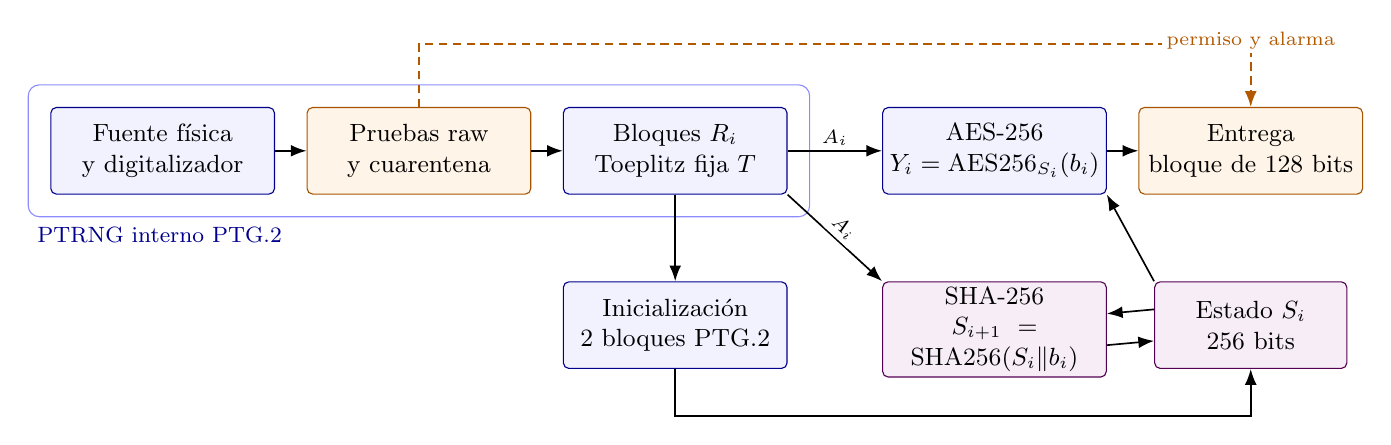
\begin{tikzpicture}[
font=\small, >=Latex, node distance=4mm,
blk/.style={draw=blue!55!black,fill=blue!5,rounded corners=2pt,align=center,
minimum height=11mm,text width=27mm,inner sep=2pt},
test/.style={blk,draw=orange!65!black,fill=orange!9},
state/.style={blk,draw=violet!65!black,fill=violet!7},
arr/.style={->,semithick},
ctl/.style={->,semithick,densely dashed,orange!70!black},
label/.style={font=\scriptsize,fill=white,inner sep=1.5pt}
]
\node[blk] (raw) {Fuente física\\y digitalizador};
\node[test,right=of raw] (health) {Pruebas raw\\y cuarentena};
\node[blk,right=of health] (toe) {Bloques $R_i$\\Toeplitz fija $T$};
\node[blk,right=12mm of toe] (aes) {AES-256\\$Y_i=\AES_{S_i}(b_i)$};
\node[test,right=of aes] (gate) {Entrega\\bloque de 128 bits};
\node[state,below=11mm of aes] (hash) {SHA-256\\$S_{i+1}=\SHA(S_i\|b_i)$};
\node[state,below=11mm of gate,text width=23mm] (reg) {Estado $S_i$\\256 bits};
\node[blk,below=11mm of toe] (seed) {Inicialización\\2 bloques PTG.2};
\draw[arr] (raw) -- (health);
\draw[arr] (health) -- (toe);
\draw[arr] (toe) -- node[label,above] {$A_i$} (aes);
\draw[arr] (aes) -- (gate);
\draw[arr] (toe.south east) -- node[label,sloped,above] {$A_i$} (hash.north west);
\draw[arr] (toe) -- (seed);
\draw[arr] (seed.south) |- ([yshift=-6mm]reg.south) -- (reg.south);
\draw[arr] (reg.north west) -- (aes.south east);
\draw[arr] ([yshift=2mm]reg.west) -- ([yshift=2mm]hash.east);
\draw[arr] ([yshift=-2mm]hash.east) -- ([yshift=-2mm]reg.west);
\draw[ctl] (health.north) -- ++(0,8mm) -| node[label,pos=.58,above] {permiso y alarma} (gate.north);
\begin{scope}[on background layer]
\node[draw=blue!45,rounded corners,fit=(raw)(health)(toe),inner sep=2.8mm] (ptgtwo) {};
\end{scope}
\node[font=\footnotesize,text=blue!55!black,anchor=north west] at (ptgtwo.south west) {PTRNG interno PTG.2};
\end{tikzpicture}
}
\caption{Arquitectura propuesta. $b_i=p\oplus A_i$ para las dos primitivas.
La rama de inicialización consume bloques propios. La entrega depende del permiso
de salud y de completar la actualización de estado.}
\label{fig:arch}
\end{figure}

\paragraph{Inicialización y reseed.}
Tras superar el start-up se generan dos bloques intermedios dedicados $B_0,B_1$
y se toma $S_0=B_0\|B_1$. Se propone el mismo reemplazo del estado para el
reseed explícito. El procedimiento espera bloques frescos, invalida material
pendiente de la época anterior y borra el estado reemplazado. Si para cada
bloque se verifica uniformemente en su historial una cota puntual de
minentropía de $128v$ bits, incluyendo $B_0$ al evaluar $B_1$, se obtiene
$\hm(B_0,B_1\mid E)\ge256v$. Para $v=0.98$ esto da $250.88$ bits y supera
los 240 de DRG.3.4. El cálculo requiere una cota para ambos bloques y sus
dependencias. Una estimación marginal separada de cada bloque no acredita
la semilla conjunta. El reseed se somete a la misma obligación de evidencia
\cite[§§161--164 y 207; §5.2.2 como ejemplo de especificación]{ais}.

\paragraph{Generación.}
Con $p\in\bits^{128}$ público, fijo y documentado, el núcleo ejecuta
\begin{align}
 b_i &=p\oplus A_i, &
 Y_i &= \AES_{S_i}(b_i), &
 S_{i+1}&=\SHA(S_i\|b_i).
 \label{eq:core}
\end{align}
AES toma $S_i$ como clave de 256 bits y $b_i$ como bloque de 128 bits.
SHA-256 recibe exactamente 384 bits antes del padding del estándar.
El perfil operativo admite una entrega de un bloque completo por comando.
Una API de lectura larga queda encima del núcleo y consume un bloque fresco por
cada bloque de salida. Se serializan las transacciones y se actualiza el estado
antes de emitir el bloque. El perfil especifica reset, fallo a mitad de
transacción, antigüedad de buffers y borrado de copias. La API PTG.3 sólo
toma $A_i$ de la ruta física calificada. Si no hay un bloque fresco validado,
se bloquea o devuelve un error. El modo autónomo ($a=\varnothing$) se analiza
para PTG.3.2 y carece de acceso desde la API de salida ITS
\cite[§§376--388 y 976, 996--998]{ais}\cite{aes,sha}.

\paragraph{Inhibición.}
Las pruebas de arranque, en línea y de fallo total observan datos raw
antes de Toeplitz. Se cuantifica el retardo máximo de detección de fallo total
en muestras, se dimensiona la cuarentena en relación con ese retardo y se
impide la entrega de bloques contaminados, incluidos los que ya estén en
tránsito. Ante fallo liberación y reseed quedan inhibidos, se invalida lo
pendiente y se requiere un arranque válido antes de servir otra época.
Se valida el comportamiento bajo inyección de fallos de la fuente y de
la canalización. Las pruebas sobre la salida complementan la evidencia de
inconspicuidad \cite[§§308--312, 326, 367 y 375]{ais}.

\section{Garantía ITS del postprocesado}

\begin{proposition}[Un bloque]
Para todo $s$, la transformación $\pi_s(a)=\AES_s(p\oplus a)$ es una
permutación de $\bits^{128}$. Con información lateral clásica $E$,
\[
\hm(Y_i\mid S_i,E)=\hm(A_i\mid S_i,E),\qquad
\dist(P_{Y_i S_i E},\ud_{128}\otimes P_{S_iE})
=\dist(P_{A_i S_i E},\ud_{128}\otimes P_{S_iE}).
\]
Aquí $\hm(X\mid Z)=-\log_2\sum_z P(z)\max_xP(x\mid z)$ y
$\dist$ es distancia de variación total.
\end{proposition}
\begin{proof}
Para cada $(s,e)$, $P(Y_i=y\mid s,e)=P(A_i=\pi_s^{-1}(y)\mid s,e)$.
Permutar las masas preserva su máximo, su entropía de Shannon y la suma de
desviaciones absolutas respecto de $2^{-128}$. En el caso cq con estado $S_i$
clásico, la permutación controlada por $S_i$ es unitaria y deja invariante el
ideal uniforme producto. Conserva la distancia de traza, y el observador
puede convertir cualquier estrategia de adivinación de $A_i$ en una de $Y_i$
y viceversa mediante $S_i$. Esto conserva $\hm$ condicional cq.
\end{proof}

\begin{proposition}[Secuencia y presupuesto de error]
Para $q$ transacciones de generación entre reseeds, fijado $S_0$, el mapa
$A^q\mapsto Y^q$ es una permutación de $\bits^{128q}$. Por tanto,
\[
\dist(P_{Y^q S_0 E},\ud_{128q}\otimes P_{S_0 E})
=\dist(P_{A^q S_0 E},\ud_{128q}\otimes P_{S_0 E}).
\]
Si para cada $i$ se dispone de
$\dist(P_{A_i A_{<i} S_0 E},\ud_{128}\otimes P_{A_{<i} S_0 E})\le\epsilon_i$,
el error conjunto está acotado por $\min(1,\sum_{i=1}^q\epsilon_i)$.
\end{proposition}
\begin{proof}
El primer inverso AES recupera $A_1$. Con él se reconstruye el siguiente
estado por SHA-256 y el procedimiento continúa. El inverso existe
aunque SHA-256 no sea inyectiva. El argumento anterior se aplica a la
permutación de la secuencia. Reemplazar cada bloque por uno uniforme en una
cadena de híbridos de prefijos reales y sufijos ideales cuesta a lo sumo
$\epsilon_i$ por bloque. Se suman las distancias por la desigualdad triangular.
\end{proof}

La prueba preserva también la minentropía conjunta condicionada a $S_0,E$.
En un horizonte que atraviesa reseeds se fija además la secuencia de materiales
de reseed si se usa el mismo inverso por épocas, o se compone aplicando un
modelo que los incluya en el historial y en la información lateral pertinente.
Si $E$ incluye copias posteriores del estado, trazas del control o selectores
derivados de los bloques, las identidades siguen comparando ambos mundos
con el mismo $E$, pero puede desaparecer la premisa de proximidad a uniforme
para $A^q$. Una cota de entropía marginal o un resultado con información
meramente causal no acredita secreto frente a tal transcript. El §402
explica por qué PTG.3 acredita la última aportación física. En modo autónomo,
$q$ salidas continuas derivadas de una única semilla de $k$ bits tienen
soporte de tamaño $\le 2^k$ cuando las demás entradas están fijadas y, para
$128q>k$, distancia a uniforme $\ge 1-2^{k-128q}$
\cite[§§390(iii), 397(ii), 402--403 y 996--998]{ais}.

Para peticiones truncadas a $\ell$ bits, la distancia a uniforme de la
proyección está acotada por el error del bloque completo, y una cota
conservadora es $\hm(\operatorname{pref}_\ell Y_i\mid S_i,E)\ge
\max(0,\hm(A_i\mid S_i,E)-(128-\ell))$. Se especifican bloques completos
en la API ITS para conservar la igualdad de minentropía. Se evita además
interpretar el padding de entradas variables del §996 como una biyección
sobre la unión de todas las longitudes \cite[§§976, 996--997]{ais}.

\section{Toeplitz y acreditación del PTG.2 interno}
\label{sec:toeplitz}

\subsection{Opción principal: matriz fija y modelo de fuente verificable}

El §342 indica que una función de hash fija permanente se trata como
postprocesado algorítmico y que su cota se deriva del modelo estocástico.
Esto habilita una Toeplitz fija, pública y versionada, al amparo de los
§§335--336 y 342. Para justificar un dispositivo se fija la matriz que
efectivamente se ejecuta, la convención de bits, el modelo condicional
y el rango de parámetros verificado. El rango completo sirve para
entradas uniformes. Para una fuente arbitraria, el soporte en el núcleo
de la matriz daría salida constante incluso con $n-128$ bits de
minentropía. Por ello una cota de minentropía bruta por sí sola resulta
insuficiente para esta ruta \cite[§§335--338 y 342]{ais}.

\paragraph{Construcción concreta bajo una hipótesis explícita.}
Para un entero $r\ge1$ se dispone el bloque raw en $r$ grupos consecutivos
de 128 bits y se fija la Toeplitz binaria
\[
T_r=\left[ I_{128}\ I_{128}\ \cdots\ I_{128}\right],\qquad
(T_r)_{u,v}=\mathbf 1\{v-u\equiv0\pmod{128}\}.
\]
Cada bit de salida es la paridad de $r$ muestras intercaladas con paso 128.
Supóngase que, dado $Z_i=(S_0,S_i,E,A_{<i})$, los $128r$ bits del bloque son
independientes y cada uno satisface
$|1-2\Pr[R_{i,j}=1\mid Z_i=z]|\le\beta$ para todo contexto admisible $z$.
No se supone que los sesgos de todos los bits sean iguales. Las paridades
usan conjuntos de muestras disjuntos y son independientes dado $z$.
Su sesgo absoluto en la convención anterior es como máximo $\beta^r$.
Por tanto se obtienen las cotas
\begin{align}
\hm(A_i\mid Z_i=z)&\ge 128\bigl[1-\log_2(1+\beta^r)\bigr],\\
\left|\Pr[A_{i,u}=1\mid Z_i=z]-\tfrac12\right|
  &\le \tfrac12\beta^r,\\
\dist(P_{A_i\mid Z_i=z},\ud_{128})
  &\le \tfrac12\sqrt{(1+\beta^{2r})^{128}-1}.
\label{eq:product}
\end{align}
Para la última desigualdad se usa
$\dist\le\tfrac12\sqrt{\chi^2}$ y la identidad
$1+\chi^2(\bigotimes_jP_j\Vert\ud_{128})
=\prod_j(1+\chi^2(P_j\Vert\ud_1))$.

Como ejemplo de dimensionamiento, $\beta=0.2$ y $r=15$ consumen 1920 bits
raw por bloque. Se obtiene $\beta^r=3.2768\cdot10^{-11}$,
un déficit de minentropía por bit $\le4.728\cdot10^{-11}<2^{-32}$
y una distancia por bloque $\le1.854\cdot10^{-10}$. El sesgo por bit
queda dentro del intervalo requerido por PTG.2.2. Estos números son
consecuencias de la hipótesis de independencia condicional y del límite
de sesgo. El modelo físico debe validar ambas hipótesis en el régimen
de operación, incluidos feedback, arranque, ambiente y telemetría.
El límite AIS de minentropía y la proximidad a uniforme para un horizonte
son claims diferentes. Por ejemplo, usando sólo esta cota, $10^6$ bloques
dan una cota superior de distancia de $1.854\cdot10^{-4}$ para ese
horizonte. Para un objetivo
$2^{-64}$ con $10^6$ bloques y las mismas hipótesis, $r=38$ es suficiente
($n=4864$). Son cotas de diseño, separadas de la confianza experimental
en los parámetros. Fijar además $S_0$ en $Z_i$ permite aplicar el argumento
de composición. El paso de $Z_i$ a $(S_0,E,A_{<i})$ preserva la cota de
distancia por convexidad.

\paragraph{Modelo con dependencia.}
Para una matriz fija general $T$ de $128$ filas se puede probar
minentropía y distancia acotando las correlaciones de paridad. Dado
un contexto clásico $z$, sea
$\gamma_v(z)=\mathbb{E}[(-1)^{(T^\top v)\cdot R_i}\mid z]$.
Inversión de Walsh y Parseval dan
\begin{align}
\max_a P(A_i=a\mid z)&\le 2^{-128}\bigl(1+\sum_{v\ne0}|\gamma_v(z)|\bigr),\notag\\
\dist(P_{A_i\mid z},\ud_{128})&\le \tfrac12\sqrt{\sum_{v\ne0}|\gamma_v(z)|^2}.
\end{align}
El sesgo por bit $u$ se controla con $|\gamma_{e_u}|/2$.
Si el modelo es Markov binario, una paridad de máscara
$w=T^\top v$ se evalúa por un producto de matrices
$\pi^\top D_{w_1} P D_{w_2}\cdots P D_{w_n}\mathbf 1$,
donde $D_b=\operatorname{diag}(1,(-1)^b)$.
Con estado oculto se sustituyen los factores por operadores de transición
y emisión del modelo pertinente. Para 128 bits enumerar todos los $v$
no es práctico. Se necesita una cota estructural uniforme, por ejemplo
por pesos de paridad o contracción, o una matriz cuya estructura haga
la suma tratable. Se deben cubrir regiones válidas de parámetros y
contextos con evidencia del modelo; probar un punto nominal no cubre
el peor caso. La prueba de producto anterior sólo se usa si el modelo
justifica sus hipótesis. En presencia de memoria fuerte, la arquitectura
sigue siendo la misma, pero la elección de $T$, $r$ y los claims
quedan sujetos a ese análisis.

\subsection{Alternativa: familia Toeplitz con selector renovado}

Una matriz Toeplitz de $128\times n$ se selecciona mediante
$d=n+127$ bits. Para la familia completa y uniformemente seleccionada,
cada diferencia raw no nula tiene probabilidad de colisión $2^{-128}$.
En efecto, la primera coordenada no nula de la diferencia fija un pivote
de semilla distinto por fila y da un sistema triangular de rango 128.
Si el selector $D_i$ es uniforme e independiente del estado cq
de $(R_i,Z_i)$ y $\hm(R_i\mid Z_i)\ge k_i$, el leftover hash lemma da
\[
\tfrac12\left\|\rho_{A_iD_iZ_i}
      -\tau_{128}\otimes\rho_{D_iZ_i}\right\|_1
\le \tfrac12 2^{(128-k_i)/2}.
\]
Una desviación del selector respecto de uniforme o una correlación con
la entrada requiere una cota adicional sobre la distribución conjunta.
Distancia media del extractor y límite de entropía para una matriz
seleccionada son obligaciones distintas. En particular, para
minentropía de un bloque de 128 bits, distancia $\epsilon$ por sí sola
da $\pg\le 2^{-128}+\epsilon$, \emph{no} una cota de 128 bits menos
$\epsilon$. En una revisión normativa debe justificarse el límite de
probabilidad de incumplir la cota por selector de §338(c), además del
sesgo y las demás condiciones. El argumento cuántico se refiere al
horizonte y la información lateral incluidos en la hipótesis cq
\cite[§§337--342, 641--648, 951--955]{ais}\cite{lhl}.

La ruta de familia universal de AIS exige selección por bloque,
secreto de índices incluso tras desinstanciación, familia de al menos
$2^{200}$ matrices, condiciones de dependencia entre índices y ley
fuerte para la cantidad de entropía evaluada, además de §338(c).
§342 permite una fuente PTG.3 con el claim indicado allí y excluye
un DRG.3 como generador de índices. Usar un DRG.3 para esos índices
no es parte de esta arquitectura. Si se elige esta alternativa,
la fuente de índices debe justificarse sin argumentación circular,
con su presupuesto de tasa, variación y dependencia física.
El carácter strong del extractor permite incluir la semilla en la
vista de la prueba matemática bajo sus hipótesis. La opción de
certificación del §338 mantiene su requisito de secreto de índices
\cite[§§338--342, 951--955]{ais}.

\section{¿Qué acredita el ejemplo DRG.3 de BSI?}
\label{sec:drg}

\subsection{Tupla y alcance de la conclusión}

Se puede citar como fundamento directo el ejemplo de los §§996--998.
Para el modo autónomo y el modo con entrada física de 128 bits, la
especialización de la 9-tupla queda así
\[
\begin{gathered}
\mathcal S=\bits^{256},\quad
\mathcal S_{\mathrm{req}}=\mathcal S\times\bits^{128},\quad
\mathcal R=\bits^{128},\quad
\mathcal A=\{\varnothing\}\cup\bits^{128},\quad I=\{128\},\\
\phi_{\mathrm{req}}(s,a)=(s,\iota(a)),\qquad
\phi_0=\operatorname{id}_{\mathcal S_{\mathrm{req}}},\\
\psi(s,u)=\AES_s(p\oplus u),\qquad
\phi(s,a)=\SHA(s\|(p\oplus\iota(a))),
\end{gathered}
\]
donde $\iota(\varnothing)=0^{128}$ e $\iota(a)=a$ cuando $|a|=128$.
La operación física se restringe a $a\in\bits^{128}$. La variante
publicada por BSI acepta $0\le |a|\le128$ y $I=\{1,\ldots,128\}$.
Ambas comparten las primitivas y su interacción, con un número interno
por petición. El estado que se conserva es de 256 bits. La salida
biyectiva respecto de $a$ no implica que la transición respecto de $s$
sea biyectiva. Para la siembra y reseed se documentan por separado
las tuplas de los procedimientos, con material $B_0\|B_1$,
sin personalización y con asignación de ese material al estado
\cite[§§127--164, 207, 976, 996--998]{ais}.

BSI califica explícitamente la construcción como DRG.3 en el §998.
Invoca la seguridad de AES-256 frente a texto elegido para los
argumentos de predecesores y sucesores y la propiedad unidireccional
de la transición para \emph{enhanced backward secrecy}.
La 9-tupla define el funcionamiento, y el §998 aporta una
justificación algorítmica de alto nivel. Para PTG.3.2, el §380
acota la referencia a DRG.3.3 y DRG.3.5--8. La evaluación del
producto tiene que ligar ese argumento a la implementación y a
su perfil operativo. Un claim autónomo DRG.3 para el producto añade
las obligaciones de inicialización, entropía y ensayos de la clase.

\subsection{Matriz de evidencias}

\begin{table}[htbp]
\centering\small
\begin{tabularx}{\linewidth}{@{}lYY@{}}
\toprule
Requisito & Base disponible & Evidencia específica de la instancia \\
\midrule
DRG.3.1, .4 & Se propone PTG.2 como origen de seed y reseed.
DRG.3.4 admite la opción TRNG con $\hm\ge240$ bits en el estado eficaz
inicial. & Especificar ambos procedimientos, acreditar el PTG.2 y la
cota conjunta de los 256 bits tras siembra y reseed. \\
DRG.3.2 & Un número interno de 128 bits por petición queda bajo
el máximo $2^{19}$. & Demostrar el límite en la API del núcleo.
La agregación de bloques queda en la API exterior. \\
DRG.3.3 & La tupla usa 256 bits de estado y AES-256 consume toda la clave.
El mínimo es 246 bits de estado eficaz. & Vincular toda la clave y
toda la entrada de SHA a la implementación, justificar estado eficaz,
ausencia de recortes, clases equivalentes relevantes o estados
operativos degenerados. \\
DRG.3.5, .6 & §998 da el argumento de sucesores y predecesores
a partir de salidas observadas. & Explicitar oráculos, transcript,
límites de peticiones, múltiples instancias y supuestos sobre AES y
su composición con la transición. \\
DRG.3.7 & §998 invoca unidireccionalidad de la transición y hay
un número interno por petición. & Analizar exposición de estado
posterior y entrada conocida, granularidad elegida y límites de
seguridad. Verificar el orden actualización/entrega y el borrado. \\
DRG.3.8 & La operación es híbrida. La interacción AES/SHA es el
punto de partida para el argumento algorítmico. & Cubrir entradas
elegidas, repetidas y nulas. Estudiar intentos de forzar colisión
o repetición de estados y claves relacionadas. La frescura del
PTG.2 no reemplaza el análisis de este requisito. \\
DRG.3.9 & AES-256 y SHA-256 son primitivas especificadas.
§998 conecta la transición con la propiedad unidireccional. &
Documentar codificación, vectores conocidos, correspondencia de
primitivas y alcance de la hipótesis de preimagen en este uso. \\
DRG.3.10 & Requisito de inconspicuidad estadística. &
Adjuntar resultados sobre el generador implementado y su modo
autónomo para un claim DRG.3 completo. \\
\bottomrule
\end{tabularx}
\caption{Desglose de DRG.3 del §207 y aplicación de §§211--214, 380 y 996--998.}
\end{table}

Los argumentos computacionales se documentan con la convención de
forward y backward secrecy de AIS. Con estado comprometido y
entrada conocida interesa la reconstrucción de salidas anteriores
(\emph{enhanced backward secrecy}). La salida AES de texto conocido
bajo claves sucesivas derivadas de SHA no está cubierta
automáticamente por un teorema PRP de clave fija.
Tampoco una definición aislada de resistencia a preimagen demuestra
por sí sola todas las propiedades conjuntas del generador.
Para justificar resistencia con entradas elegidas se describe
el juego de ataque y qué datos, estados y entradas puede observar
o fijar el adversario. Se analiza si puede distinguir, predecir,
repetir o dirigir la evolución y qué papel tienen las colisiones o
sesgos del estado durante la vida útil. Como referencia analítica,
se puede separar un modelo de cifrado ideal por clave y uno de
transición ideal sobre entradas $s\|b$ y estudiar consultas,
repeticiones y exposición de estado, dejando expresas las
hipótesis al pasar a AES/SHA concretos. La prueba ITS de la
permutación permanece exacta con independencia de ese análisis.
Los §§121--125 exigen examinar fuerza y evolución del estado
eficaz, y §211 exige que las propiedades sean algorítmicas.
Para un único bloque de 128 bits la referencia de adivinación ciega
es $2^{-128}$ por intento. El umbral de 240 bits de DRG.3.4 se aplica
a la minentropía del estado eficaz inicial
\cite[§§121--125, 195, 207, 211--214 y 998]{ais}.

\section{Matriz de evaluación PTG.3}

\begin{table}[htbp]
\centering\small
\begin{tabularx}{\linewidth}{@{}lY@{}}
\toprule
Requisito & Evidencia y criterio para esta arquitectura \\
\midrule
PTG.3.1 & Modelo y validación de la estacionariedad local raw en el
dominio de operación. Delimitar digitalizador y feedback. \\
PTG.3.2 & Núcleo con memoria que implementa §§996--998.
Dossier de DRG.3.3 y DRG.3.5--8, con análisis autónomo.
El bloque físico afecta también al estado siguiente. \\
PTG.3.3 & Dossier PTG.2 del bloque completo fuente--pruebas--Toeplitz.
Acreditar 128 bits intermedios por transacción y la ruta física a
la entrada adicional. \\
PTG.3.4 & Un bloque intermedio nuevo de 128 bits por cada bloque
de salida de 128 bits, como en §390(iii). Probar consumo único,
ausencia de fallback y que inicialización/reseed son consumos
adicionales de la fuente. \\
PTG.3.5 & Claim concreto de minentropía de salida, sustentado por
la cota del PTRNG interno y la permutación. Registrar por separado
la vista $E$, el horizonte y el error ITS que se quiera declarar. \\
PTG.3.6--.8 & Tests sobre raw, evidencia de tiempos de detección,
cuarentena y puerta de salida. Probar bloqueo ante fallos,
retorno controlado de una época y ausencia de bypass. \\
PTG.3.9 & Inconspicuidad estadística de la salida interna y
resultados documentados. Para el PTG.2, además, adjuntar las
comprobaciones de PTG.2.2 y la suite $T_{\mathrm{irn}}$ de PTG.2.6. \\
\bottomrule
\end{tabularx}
\caption{Mapa del SFR PTG.3 del §375 hacia evidencias del diseño y del producto.}
\end{table}

\section{Conclusión}

La arquitectura a evaluar es un PTG.2 que produce bloques de 128 bits
físicos mediante Toeplitz y un postprocesado AES/SHA con estado que
consume exactamente uno por salida. La evidencia decisiva es la cota
condicional de la fuente tras Toeplitz. El núcleo de BSI la conserva sin
degradación para bloques completos, incluso si el estado de esa llamada
es conocido en el modelo ITS. La referencia ofrece la construcción y el
argumento algorítmico DRG.3. Los modelos de fuente y amenaza, las pruebas
físicas, el perfil de estado y las verificaciones de implementación
completan el expediente requerido para una decisión de conformidad.

\begingroup\small
\begin{thebibliography}{9}
\setlength{\itemsep}{2pt}
\bibitem{ais} M. Peter y W. Schindler. \emph{A Proposal for Functionality
Classes for Random Number Generators}, v3.0, BSI, 10 de septiembre de 2024.
Referencia matemática-técnica común de AIS 20 y AIS 31. Versión cotejada
el 20 de noviembre de 2026.
\href{https://www.bsi.bund.de/SharedDocs/Downloads/EN/BSI/Certification/Interpretations/AIS_31_Functionality_classes_for_random_number_generators_e_2024.pdf?__blob=publicationFile\&v=3}{PDF oficial}.
\bibitem{lhl} M. Tomamichel, C. Schaffner, A. Smith y R. Renner.
Leftover Hashing Against Quantum Side Information.
\emph{IEEE Transactions on Information Theory}, 57(8), 2011.
\href{https://arxiv.org/abs/1002.2436}{arXiv:1002.2436}.
\bibitem{aes} NIST. \emph{Advanced Encryption Standard (AES)}.
FIPS 197, actualización editorial de 2023.
\url{https://doi.org/10.6028/NIST.FIPS.197-upd1}.
\bibitem{sha} NIST. \emph{Secure Hash Standard (SHS)}.
FIPS 180-4, 2015. \url{https://doi.org/10.6028/NIST.FIPS.180-4}.
\end{thebibliography}
\endgroup
\end{document}
